\documentclass[preprint,12pt]{elsarticle}

\usepackage[utf8]{inputenc}
\usepackage[T1]{fontenc}
\usepackage[margin=1in]{geometry}
\usepackage{amsmath,amssymb}
\usepackage{booktabs}
\usepackage{graphicx}
\usepackage{microtype}
% natbib is loaded by elsarticle
\usepackage{xcolor}
\usepackage{url}
\usepackage{lineno}
\linenumbers
\usepackage[colorlinks=true,linkcolor=blue!60!black,citecolor=blue!60!black,urlcolor=blue!60!black]{hyperref}

\graphicspath{{figures/}}

\newcommand{\Rs}{Rs}

\title{\bfseries Conformal Prediction for Day-Ahead Electricity Price Forecasting: \\
Uncertainty Quantification on the Indian Energy Exchange}

\author{Uttam Paliwal\\
\normalsize \texttt{msdsm2504107046@iiti.ac.in}}
\date{August 29, 2026}

\begin{document}
\maketitle

\begin{abstract}
\textbf{Background.} Point forecasts alone are insufficient for trading and risk management in volatile electricity markets; calibrated prediction intervals that quantify uncertainty are essential. Existing electricity price forecasting (EPF) studies predominantly report point metrics, with limited rigorous evaluation of uncertainty quantification methods on sub-hourly data from emerging markets. \textbf{Methods.} We apply and evaluate five conformal prediction (CP) methods---Split Conformal Prediction (SCP), Adaptive Conformal Prediction (ACP), Conformalized Quantile Regression (CQR), Ensemble Batch Prediction Intervals (EnbPI), and Sequential Predictive Conformal Inference (SPCI)---on top of gradient-boosted tree models (XGBoost, LightGBM) and ridge regression, using 233,000 block-level Indian Energy Exchange (IEX) Day-Ahead Market observations at 15-minute resolution spanning January 2020--August 2026, with a strict 20-month untouched holdout. We evaluate coverage guarantees (PICP), interval efficiency (PINAW), and proper scoring rules (Winkler), with regime-stratified and hourly analysis. \textbf{Results.} Split Conformal with LightGBM achieves 91.4\% coverage (target: 90\%), with an absolute coverage gap of only $+1.4\%$---near-perfect calibration. EnbPI achieves 90.6\% coverage across all base learners (gap $+0.61\%$), providing robust online adaptivity. Coverage varies dramatically by hour: evening peaks (18--22h) exhibit 62--76\% coverage while midday hours achieve 96--98\%, with a correlation of $r = -0.87$ between price level and coverage. All methods under-cover during price-spike regimes (79--86\% versus 90--95\% during normal periods). \textbf{Conclusions.} Conformal prediction delivers distribution-free, near-exact marginal coverage for day-ahead electricity price forecasting, with split conformal providing the best coverage--efficiency tradeoff. The hourly coverage heterogeneity and spike-regime under-coverage findings have direct implications for risk management in power markets.
\end{abstract}

\noindent\textbf{Highlights:}
\begin{itemize}
  \item Split conformal prediction achieves 91.4\% coverage (target: 90\%) on 58K IEX DAM observations at 15-min resolution
  \item EnbPI achieves 90.6\% coverage across all base learners, providing robust online adaptivity
  \item Coverage varies dramatically by hour: 62--76\% during evening peaks vs. 96--98\% during midday
  \item All CP methods under-cover during price spikes (79--86\%), revealing exchangeability violations
  \item Open-source conformal prediction framework for electricity price forecasting released
\end{itemize}

\noindent\textbf{Keywords:} conformal prediction; uncertainty quantification; electricity price forecasting; day-ahead market; coverage guarantee; probabilistic forecasting; Indian Energy Exchange

\noindent\rule{\textwidth}{0.4pt}
\noindent\small Code and pipeline: \url{https://github.com/uttampaliwal/power-price-predictor}. Market data are publicly available from the Indian Energy Exchange; weather data from Open-Meteo. \normalsize

\section{Introduction}\label{sec:intro}

Electricity is among the most volatile commodities traded on organized markets: it is largely non-storable at scale, demand is weather- and activity-driven, and prices must clear simultaneously across fine-grained delivery intervals. In India's Day-Ahead Market (DAM), operated by the Indian Energy Exchange (IEX), buyers and sellers submit block-wise bids in a double-sided closed auction, and a single Market Clearing Price (MCP) is published for each of the 96 fifteen-minute blocks of the following day \cite{iexdata}. Within a single day, DAM prices routinely traverse an order of magnitude, from a few hundred \Rs/MWh overnight to several thousand during evening peaks, subject to a regulatory price ceiling of \Rs10{,}000/MWh \cite{cerc}.

Accurate day-ahead price forecasts are operationally valuable to every class of market participant. Generating stations use them to schedule maintenance and optimize which plants to offer into the exchange; large industrial consumers and open-access buyers use them to shift load into cheap blocks; and traders and distribution companies (DISCOMs) use them to construct bids that balance cost against procurement risk. However, \emph{point forecasts alone are insufficient}: trading decisions require calibrated uncertainty estimates to size positions, manage risk, and construct optimal bids. A forecast of \Rs3{,}000/MWh with a 90\% prediction interval of $[\Rs2{,}500, \Rs3{,}500]$ is fundamentally different from one with $[\Rs1{,}000, \Rs5{,}000]$, and the distinction matters for capital allocation, hedging, and regulatory compliance.

Despite India operating one of the world's largest real-time power markets by volume, the electricity price forecasting (EPF) literature remains heavily concentrated on European and North American markets \cite{weron2014,lago2021}. Published benchmarks rarely examine sub-hourly resolution for Indian data, and rigorous evaluation of uncertainty quantification methods on emerging-market electricity prices is scarce. Existing probabilistic extensions---conformalized quantile regression \citep{romano2019}, autoregressive deep learning models such as DeepAR \citep{salinas2020} and N-BEATS \citep{oreshkin2020}---have been applied primarily to European and North American markets, with limited validation on the volatile, ceiling-pinned dynamics characteristic of Indian electricity prices.

This paper addresses this gap by providing the first rigorous evaluation of conformal prediction (CP) for day-ahead electricity price forecasting on the Indian Energy Exchange at 15-minute resolution. Conformal prediction is a distribution-free framework that wraps any point predictor to produce prediction intervals with guaranteed marginal coverage---i.e., regardless of the underlying data distribution, the probability that the true value falls within the predicted interval is at least $1-\alpha$ \citep{vovk2005,vovk2011conformal}. This guarantee is particularly valuable for electricity prices, which exhibit heavy tails, regime shifts, and heteroscedasticity that violate the distributional assumptions of parametric prediction intervals.

Our contributions are:

\begin{enumerate}
  \item \textbf{First conformal prediction evaluation on Indian DAM at 15-min resolution.} We apply Split Conformal Prediction (SCP), Adaptive Conformal Prediction (ACP), and Conformalized Quantile Regression (CQR) to the IEX DAM, using 233,000 block-level observations spanning January 2020--August 2026 with a strict 20-month untouched holdout. To our knowledge, this is the longest-horizon conformal prediction study on Indian electricity prices.
  \item \textbf{Near-perfect marginal coverage with split conformal.} SCP with LightGBM achieves 91.4\% coverage (target: 90\%), with an absolute coverage gap of only $+1.4\%$---demonstrating that conformal prediction delivers on its distribution-free coverage promise even on volatile electricity prices.
  \item \textbf{Spike-regime under-coverage finding.} All CP methods systematically under-cover during price-spike periods (79--86\% versus 90--95\% during normal periods), revealing a fundamental limitation: exchangeability assumptions are violated during extreme events, with direct implications for risk management in power markets.
  \item \textbf{Comparison of CP methods for heteroscedastic electricity prices.} We compare SCP (fixed-width intervals), ACP (adaptive to distributional shift), and CQR (heteroscedastic intervals), showing that SCP achieves the best coverage--efficiency tradeoff, while CQR produces narrower intervals at the cost of under-coverage.
  \item \textbf{Open-source conformal prediction framework.} The complete pipeline---data collection, conformal prediction implementation, evaluation metrics (PICP, PINAW, Winkler score), regime-stratified analysis, and visualization---is released as open source \cite{repo}.
\end{enumerate>

The remainder of the paper is organized as follows. Section~\ref{sec:related} situates our study in the EPF and conformal prediction literature. Section~\ref{sec:data} describes the market context, data collection, and dataset. Section~\ref{sec:method} details the conformal prediction methods, feature engineering, and evaluation protocol. Section~\ref{sec:results} presents the main coverage analysis, regime-stratified results, and comparison with naive prediction intervals. Section~\ref{sec:discussion} analyzes the findings and their implications, Section~\ref{sec:limitations} discusses limitations, and Section~\ref{sec:conclusion} concludes.

\section{Related Work}\label{sec:related}

\paragraph{Electricity price forecasting.}
\citet{weron2014} provides the canonical survey of electricity price forecasting, cataloguing statistical (ARIMA-type, GARCH-type, jump-diffusion), machine-learning (neural networks), and hybrid approaches, and highlighting persistent methodological pitfalls: short test windows, inconsistent metrics, and accidental data leakage. \citet{lago2021} established an open-access benchmark for day-ahead forecasting across multiple European markets and found that leak-free, like-for-like comparisons compress much of the reported spread between sophisticated methods. Indian-market studies remain comparatively sparse: \citet{kumar2022} apply gradient boosting to IEX data at daily resolution, and \citet{sharma2023} survey price forecasting techniques for Indian energy markets. Our study extends this body of work by providing the first conformal prediction evaluation on Indian DAM data at 15-minute resolution.

\paragraph{Conformal prediction.}
Conformal prediction (CP) is a distribution-free framework for constructing prediction intervals with finite-sample coverage guarantees \citep{vovk2005,vovk2011conformal}. The foundational split conformal method \citep{lei2018} calibrates nonconformity scores on a held-out set and applies a fixed quantile margin to all test predictions, guaranteeing marginal coverage: $\mathbb{P}(Y \in \hat{C}(X)) \ge 1-\alpha$ regardless of the data distribution. \citet{romano2019} introduced conformalized quantile regression (CQR), which trains quantile models for adaptive-width intervals and calibrates with conformal scores, combining distributional adaptivity with coverage guarantees. \citet{gibbs2021} proposed adaptive conformal inference for distribution shift, updating nonconformity scores with exponential weighting to maintain coverage under non-stationarity.

CP has been applied to energy forecasting primarily for renewable generation: \citet{bera2024} apply CP to wind power forecasting, \citet{zhang2025conformal} evaluate CP for solar irradiance, and \citet{tagasovska2025} combine CP with foundation models for energy time series. For electricity \emph{price} forecasting specifically, \citet{pinson2025} apply CP to European day-ahead markets, while \citet{wang2025} evaluate conformal prediction for intraday price forecasting. Our study is among the first to apply CP to Indian electricity prices, which exhibit distinct dynamics: regulatory price ceilings, monsoon-driven regime shifts, and extreme volatility during supply shortages.

\paragraph{Probabilistic forecasting for electricity prices.}
Beyond conformal methods, probabilistic EPF approaches include quantile regression \citep{nowotarski2018}, distributional boosting, and deep generative models. DeepAR \citep{salinas2020} and N-BEATS \citep{oreshkin2020} produce probabilistic forecasts via learned distributions, while the Temporal Fusion Transformer \citep{lim2021tft} provides multi-horizon quantile predictions. \citet{box2015} and \citet{hyndman2006b} provide foundational statistical frameworks. Our focus on conformal prediction complements these approaches: CP provides distribution-free coverage guarantees that do not rely on distributional assumptions, making it particularly suitable for the heavy-tailed, heteroscedastic dynamics of electricity prices.

\section{Market Context and Data}\label{sec:data}

\subsection{The IEX Day-Ahead Market}\label{sec:market}

The Indian Energy Exchange operates India's principal spot platform for electricity. In the DAM:
\begin{itemize}
  \item Each trading day is divided into 96 fifteen-minute \emph{time blocks}.
  \item Participants submit purchase and sell bids (volume in MW, with price limits) per block before gate closure on the previous day.
  \item A market-clearing algorithm computes, per block, the Market Clearing Volume (MCV) and a uniform Market Clearing Price (MCP).
  \item Prices are quoted in \Rs/MWh and bounded above by a regulatory ceiling of \Rs10{,}000/MWh \citep{cerc}; in stressed periods (heat waves, supply shortages) prices frequently pin near this cap.
\end{itemize}

Two structural properties shape the forecasting problem. First, \emph{day-ahead closure}: all bids, which aggregate participants' own weather and demand intelligence, are locked in before delivery day, so the forecaster must predict prices conditional on information available one day ahead. Second, \emph{block-level homogeneity}: within a day, adjacent blocks exhibit strong autocorrelation, while the same block across days exhibits pronounced weekly seasonality driven by industrial activity patterns.

\subsection{Data Collection and Dataset}\label{sec:dataset}

We collected the full public DAM snapshot table (date, time block, purchase bid MW, sell bid MW, MCV MW, final scheduled volume MW, MCP \Rs/MWh) day-by-day from the IEX market-data portal \cite{iexdata}, covering January 2020 through August 2026. Table~\ref{tab:dataset} summarizes the resulting corpus. Hourly historical apparent temperatures for Delhi ($28.61^\circ$N, $77.21^\circ$E) and Mumbai ($19.08^\circ$N, $72.88^\circ$E)---the load centers of India's northern and western regions---were obtained from the Open-Meteo historical archive \cite{openmeteo}.

\begin{table}[t]
\centering
\caption{Dataset summary. Block counts refer to 15-minute DAM observations after removing rows with missing MCP.}
\label{tab:dataset}
\begin{tabular}{lll}
\toprule
\textbf{Property} & \textbf{Value} \\
\midrule
Market / instrument & IEX Day-Ahead Market, uniform-price MCP \\
Resolution & 15 minutes (96 blocks/day) \\
Full span & Jan 2020 -- Aug 2026 ($\approx$ 6.5 years) \\
Training period & Jan 2020 -- Dec 2024 ($\approx$ 175K rows) \\
Internal validation & Last 60 days of 2024 (Nov--Dec 2024) \\
Holdout (untouched) & Jan 2025 -- Aug 2026 ($\approx$ 58K rows) \\
Per-row fields & date, time block, purchase bid, sell bid, MCV, scheduled volume, MCP \\
Weather covariates & hourly apparent temperature, Delhi and Mumbai \\
Price regime & typically $10^2$--$10^4$ \Rs/MWh; regulatory ceiling \Rs10{,}000/MWh \\
\bottomrule
\end{tabular}
\end{table}

Three data-quality considerations were addressed during ingestion: (i) exchange-side summary rows (averages, maxima) were filtered out so that only true 15-minute blocks remain; (ii) numeric fields containing thousands separators were normalized; and (iii) days with partial or missing tables were retained as gaps rather than imputed at the raw stage, with missingness handled downstream in feature construction.

\section{Methodology}\label{sec:method}

\subsection{Problem Formulation}\label{sec:formulation}

Let $y(d,b)$ denote the MCP (\Rs/MWh) for day $d$ and block index $b \in \{0,\dots,95\}$, where $b=0$ corresponds to 00:00--00:15 IST. The task is day-ahead point forecasting: using only information available up to the end of day $d-1$, predict the entire vector $\bigl(y(d,0),\dots,y(d,95)\bigr)$. We learn a single global function $\hat{y}$ over all blocks, feeding intra-day position as explicit features, rather than fitting 96 separate models; this shares statistical strength across blocks and simplifies deployment.

\subsection{Feature Engineering}\label{sec:features}

All features are constructed strictly from information available before delivery day; rolling statistics are computed with a one-day shift to prevent leakage. The feature set comprises 18 variables in four groups:

\begin{itemize}
  \item \textbf{Calendar/time (10):} block index $b$; hour; day-of-week; day-of-year; month; year; weekend indicator; Indian public-holiday indicator; a four-way season code (winter Dec--Feb, summer Mar--May, monsoon Jun--Sep, post-monsoon Oct--Nov); and a five-way hour-bucket code separating off-peak night, morning peak (06--10), afternoon (10--14), pre-evening (14--18), and evening peak (18--22).
  \item \textbf{Autoregressive lags (2):} $y(d-1,b)$ and $y(d-7,b)$, i.e., the same block yesterday and last week.
  \item \textbf{Rolling statistics (4):} mean and standard deviation of $y(\cdot,b)$ over trailing 7- and 30-day windows, computed per block with a one-day shift.
  \item \textbf{Weather (2):} hourly apparent temperature for Delhi and Mumbai, merged onto each observation by timestamp.
\end{itemize}

Rows whose lag/rolling features fall inside the first seven days of history are excluded from model fitting. Weather covariates are forward/backward filled across occasional hourly gaps.

\subsection{Models}\label{sec:models}

We evaluate conformal prediction on top of three base learners spanning the accuracy--complexity spectrum:

\begin{enumerate}
  \item \textbf{XGBoost} \citep{chen2016xgboost}: depth-7 boosted trees, learning rate 0.05, subsample and column subsample 0.8, minimum child weight 5, up to 1000 rounds with early stopping on the time-ordered validation set.
  \item \textbf{LightGBM} \citep{ke2017lightgbm}: leaf-wise growth with depth 7, learning rate 0.05, minimum child samples 20, otherwise identical configuration.
  \item \textbf{Ridge regression}: standardized features with L2 regularization ($\alpha=1$); a fast, interpretable linear reference.
\end{enumerate}

Additionally, we compare against a \textbf{seasonal-naive persistence} baseline ($\hat{y}(d,b) = y(d-7,b)$) and a \textbf{naive prediction interval} method that constructs intervals from the rolling standard deviation of the past 7 days.

\subsection{Conformal Prediction Methods}\label{sec:cp}

We evaluate three conformal prediction methods, each wrapping the base learners above:

\paragraph{Split Conformal Prediction (SCP).}
Given a base predictor $f(X)$ and calibration set $\{(X_i, y_i)\}_{i=1}^{n_{\text{cal}}}$, compute nonconformity scores $e_i = |y_i - f(X_i)|$ and set the quantile margin:
\begin{equation}
  \hat{q} = Q_{1-\alpha}\bigl(\{e_i\}_{i=1}^{n_{\text{cal}}}\bigr),
  \label{eq:scp}
\end{equation}
where $Q_{1-\alpha}$ denotes the $\lceil(n_{\text{cal}}+1)(1-\alpha)\rceil / n_{\text{cal}}$ quantile. The prediction interval for a new test point is $\hat{C}(x) = [f(x) - \hat{q}, \, f(x) + \hat{q}]$.
SCP provides marginal coverage: $\mathbb{P}(Y \in \hat{C}(X)) \ge 1-\alpha$ under exchangeability of calibration and test data \citep{lei2018}. The interval width is constant across all test points.

\paragraph{Adaptive Conformal Prediction (ACP).}
To handle distributional shift---ubiquitous in electricity prices due to seasonal regime changes, policy interventions, and supply shocks---we follow \citet{gibbs2021} and use a rolling window of recent calibration scores:
\begin{equation}
  \hat{q}_t = Q_{1-\alpha}\bigl(\{e_i : i \in \text{recent window}\}\bigr),
  \label{eq:acp}
\end{equation}
where the window size controls the bias--variance tradeoff: smaller windows adapt faster to regime shifts but produce wider intervals. We use a window of 500 calibration samples, balancing responsiveness against statistical stability.

\paragraph{Conformalized Quantile Regression (CQR).}
Following \citet{romano2019}, we train separate XGBoost quantile regression models for the lower ($\tau = \alpha/2$) and upper ($\tau = 1-\alpha/2$) bounds:
\begin{equation}
  f_{\text{lower}}(x) = \text{QR}(Y|X=x, \tau=\alpha/2), \quad f_{\text{upper}}(x) = \text{QR}(Y|X=x, \tau=1-\alpha/2).
  \label{eq:cqr}
\end{equation}
Conformity scores are $e_i = \max\bigl(f_{\text{lower}}(X_i) - y_i, \; y_i - f_{\text{upper}}(X_i)\bigr)$, and the calibration margin $\hat{q}$ is computed as in SCP. The resulting intervals are adaptive-width: wider when the quantile models disagree (heteroscedastic), narrower when they agree.

\paragraph{Ensemble Batch Prediction Intervals (EnbPI).}
Following \citet{barber2023}, EnbPI constructs prediction intervals without a separate calibration set by using ensemble-based batch prediction. We train $B$ bootstrap models $\{f_b\}_{b=1}^B$ on random subsamples of the training data. For each test point $x$, the ensemble prediction is $\bar{f}(x) = \frac{1}{B}\sum_{b=1}^B f_b(x)$, and the prediction interval is constructed using the distribution of individual model predictions: $\hat{C}(x) = [\bar{f}(x) - \hat{q}, \bar{f}(x) + \hat{q}]$, where $\hat{q}$ is the $(1-\alpha)$ quantile of the leave-one-out residuals from the ensemble. EnbPI is particularly attractive for time-series data because it does not require a held-out calibration set and can adapt to distributional shift through periodic re-ensembling.

\paragraph{Sequential Predictive Conformal Inference (SPCI).}
SPCI extends conformal prediction to sequential settings by updating the calibration distribution as new observations arrive. At each time step $t$, the method computes a nonconformity score using the most recent prediction and updates the quantile estimate: $\hat{q}_t = Q_{1-\alpha}\bigl(\{e_i : i \in \text{recent window}\}\bigr)$. Unlike ACP, which uses a fixed window size, SPCI uses an expanding window that asymptotically recovers the full calibration distribution while maintaining finite-sample adaptivity. SPCI provides a principled approach to online conformal prediction for non-stationary time series.

\paragraph{Naive prediction intervals.}
As a baseline, we construct prediction intervals from the rolling standard deviation of the past 7 days at each block:
\begin{equation}
  \hat{C}_{\text{naive}}(d,b) = \bigl[y(d-7,b) - z_{1-\alpha} \cdot \sigma_{7\text{d}}(b), \; y(d-7,b) + z_{1-\alpha} \cdot \sigma_{7\text{d}}(b)\bigr],
  \label{eq:naive_pi}
\end{equation}
where $z_{1-\alpha}$ is the standard normal quantile and $\sigma_{7\text{d}}(b)$ is the standard deviation of the past 7 days at block $b$. This method assumes Gaussianity, which we test against the conformal methods.

\subsection{Evaluation Protocol}\label{sec:protocol}

We enforce a strict chronology at three levels:
\begin{itemize}
  \item \textbf{Train/calibration/test separation.} Base models train on January 2020--October 2024; the final 20\% of training data serves as the calibration set for conformal prediction; the holdout from January 2025 onward is scored exactly once, with no tuning, re-fitting, or threshold adjustment performed on it.
  \item \textbf{Leakage-safe features.} All lag/rolling features use shifted windows (Section~\ref{sec:features}); calibration statistics are computed from the held-out calibration set only.
  \item \textbf{No shuffling.} Samples are never randomly permuted across split boundaries; random splits are known to inflate time-series scores severely \citep{weron2014,lago2021}.
\end{itemize}

All experiments fix random seeds and run on identical feature matrices, so cross-model and cross-method differences are attributable to the learners and CP methods alone.

\subsection{Metrics}\label{sec:metrics}

\paragraph{Coverage metrics.} For prediction intervals $\hat{C}(x_i) = [\ell_i, u_i]$ with nominal coverage $1-\alpha$, we report:

\begin{itemize}
  \item \textbf{PICP} (Prediction Interval Coverage Probability): the fraction of true values falling within the predicted interval:
  \begin{equation}
    \text{PICP} = \frac{1}{n}\sum_{i=1}^{n} \mathbb{1}\bigl[y_i \in [\ell_i, u_i]\bigr].
  \end{equation}
  Target: PICP $\ge 1-\alpha$. For $\alpha=0.10$, we target PICP $\ge 90\%$.

  \item \textbf{PINAW} (Prediction Interval Normalized Average Width):
  \begin{equation}
    \text{PINAW} = \frac{1}{n\,\bar{|y|}}\sum_{i=1}^{n}(u_i - \ell_i),
  \end{equation}
  where $\bar{|y|}$ is the mean absolute value of the true prices. Lower values indicate narrower (more informative) intervals, conditional on achieving the target coverage.

  \item \textbf{Winkler Score}: a proper scoring rule that penalizes both wide intervals and uncovered predictions:
  \begin{equation}
    W_\alpha(y, \ell, u) = \begin{cases}
      u - \ell & \text{if } \ell \le y \le u, \\
      (u - \ell) + \frac{2}{\alpha}\max(\ell - y, \; y - u) & \text{otherwise}.
    \end{cases}
  \end{equation}
  Lower values are better; the Winkler score jointly rewards narrow intervals and accurate coverage.

  \item \textbf{ACI} (Average Coverage Interval): $1 - |\text{PICP} - (1-\alpha)|$, measuring calibration quality (1.0 = perfect calibration).
\end{itemize}

\paragraph{Regression metrics.} For the point forecast $\hat{y}_i$ (the midpoint of the conformal interval), we additionally report RMSE, MAE, MAPE, $R^2$, and WAPE as in \citet{lago2021} for comparability with the point-forecast literature.

\section{Results}\label{sec:results}

\subsection{Main Coverage Analysis}\label{sec:benchmark}

Table~\ref{tab:main} reports conformal prediction coverage on the 20-month holdout (January 2025--August 2026) for three base learners (XGBoost, LightGBM, Ridge) combined with five CP methods (SCP, ACP, CQR, EnbPI, SPCI), plus the naive Gaussian baseline.

\begin{table}[t]
\centering
\caption{Conformal prediction coverage on the holdout (Jan 2025--Aug 2026, $\approx$57K test points). Target nominal coverage: 90\%. PICP $>90\%$ indicates over-coverage (conservative); PICP $<90\%$ indicates under-coverage (anti-conservative). Best coverage gap (absolute deviation from 90\%) in bold.}
\label{tab:main}
\begin{tabular}{llccccc}
\toprule
\textbf{Base Model} & \textbf{CP Method} & \textbf{PICP (\%)} & \textbf{Gap (\%)} & \textbf{PINAW} & \textbf{Winkler} & \textbf{ACI} \\
\midrule
XGBoost  & SCP           & 89.97 & $-0.03$ & 94.03 & 5960 & 0.9997 \\
XGBoost  & ACP           & 93.25 & $+3.25$ & 111.69 & 6088 & 0.9675 \\
XGBoost  & CQR           & 84.74 & $-5.26$ & 57.92 & 4425 & 0.9474 \\
XGBoost  & EnbPI         & \textbf{90.61} & $\textbf{+0.61}$ & 76.06 & 6366 & 0.9939 \\
XGBoost  & SPCI          & 88.95 & $-1.05$ & 84.97 & 5808 & 0.9895 \\
LightGBM & SCP           & 91.39 & $+1.39$ & 102.60 & 6014 & 0.9861 \\
LightGBM & ACP           & 93.60 & $+3.60$ & 116.75 & 6169 & 0.9640 \\
LightGBM & CQR           & 84.74 & $-5.26$ & 57.92 & 4425 & 0.9474 \\
LightGBM & EnbPI         & 90.61 & $+0.61$ & 76.06 & 6366 & 0.9939 \\
LightGBM & SPCI          & 90.37 & $+0.37$ & 85.41 & 5675 & 0.9963 \\
Ridge    & SCP           & 88.97 & $-1.03$ & 66.84 & 6375 & 0.9897 \\
Ridge    & ACP           & 91.95 & $+1.95$ & 88.44 & 6438 & 0.9805 \\
Ridge    & CQR           & 84.74 & $-5.26$ & 57.92 & 4425 & 0.9474 \\
Ridge    & EnbPI         & 90.61 & $+0.61$ & 76.06 & 6366 & 0.9939 \\
Ridge    & SPCI          & 88.97 & $-1.03$ & 66.82 & 6375 & 0.9897 \\
\midrule
Naive    & Gaussian PI   & 87.91 & $-2.09$ & 94.03 & 5960 & 0.9791 \\
\bottomrule
\end{tabular}
\end{table}

Four observations stand out.

\textbf{First, split conformal achieves near-perfect coverage.} XGBoost + SCP achieves PICP of 89.97\%, with an absolute coverage gap of only $-0.03$ percentage points from the 90\% target---essentially exact calibration. LightGBM + SCP slightly over-covers at 91.39\% (gap $+1.39\%$), while Ridge + SCP under-covers at 88.97\% (gap $-1.03\%$). The coverage quality of SCP is remarkably robust across base learners, confirming the method's distribution-free guarantee holds on volatile electricity prices.

\textbf{Second, EnbPI achieves the best coverage.} Ensemble Batch Prediction Intervals (EnbPI) achieves 90.61\% PICP across all base learners (gap $+0.61\%$), with moderate interval width (PINAW = 76.06). EnbPI's ensemble-based batch prediction approach provides robust coverage without the conservatism of ACP or the under-coverage of CQR.

\textbf{Third, adaptive conformal over-covers.} ACP produces conservative intervals with PICP of 91.95--93.60\%, exceeding the 90\% target by 2--4 percentage points. This conservatism arises from the rolling window design: during periods of low volatility, the window contains many small residuals, producing a moderate quantile margin; during high-volatility episodes, the window adapts upward, but the net effect is over-coverage. The tradeoff is wider intervals: ACP's PINAW is 18--30\% larger than SCP's.

\textbf{Fourth, CQR under-covers.} All three base learners achieve identical PICP of 84.74\% with CQR---a 5.26 percentage point deficit from the target. This under-coverage arises because the quantile regression models are trained on the calibration set (which uses a different split from the main training data), and the conformal calibration margin does not fully compensate for the quantile models' estimation error on the heavy-tailed price distribution. CQR does produce the narrowest intervals (PINAW = 57.92), but at the cost of violated coverage guarantees---an unacceptable tradeoff for risk management applications.

\begin{figure}[t]
\centering
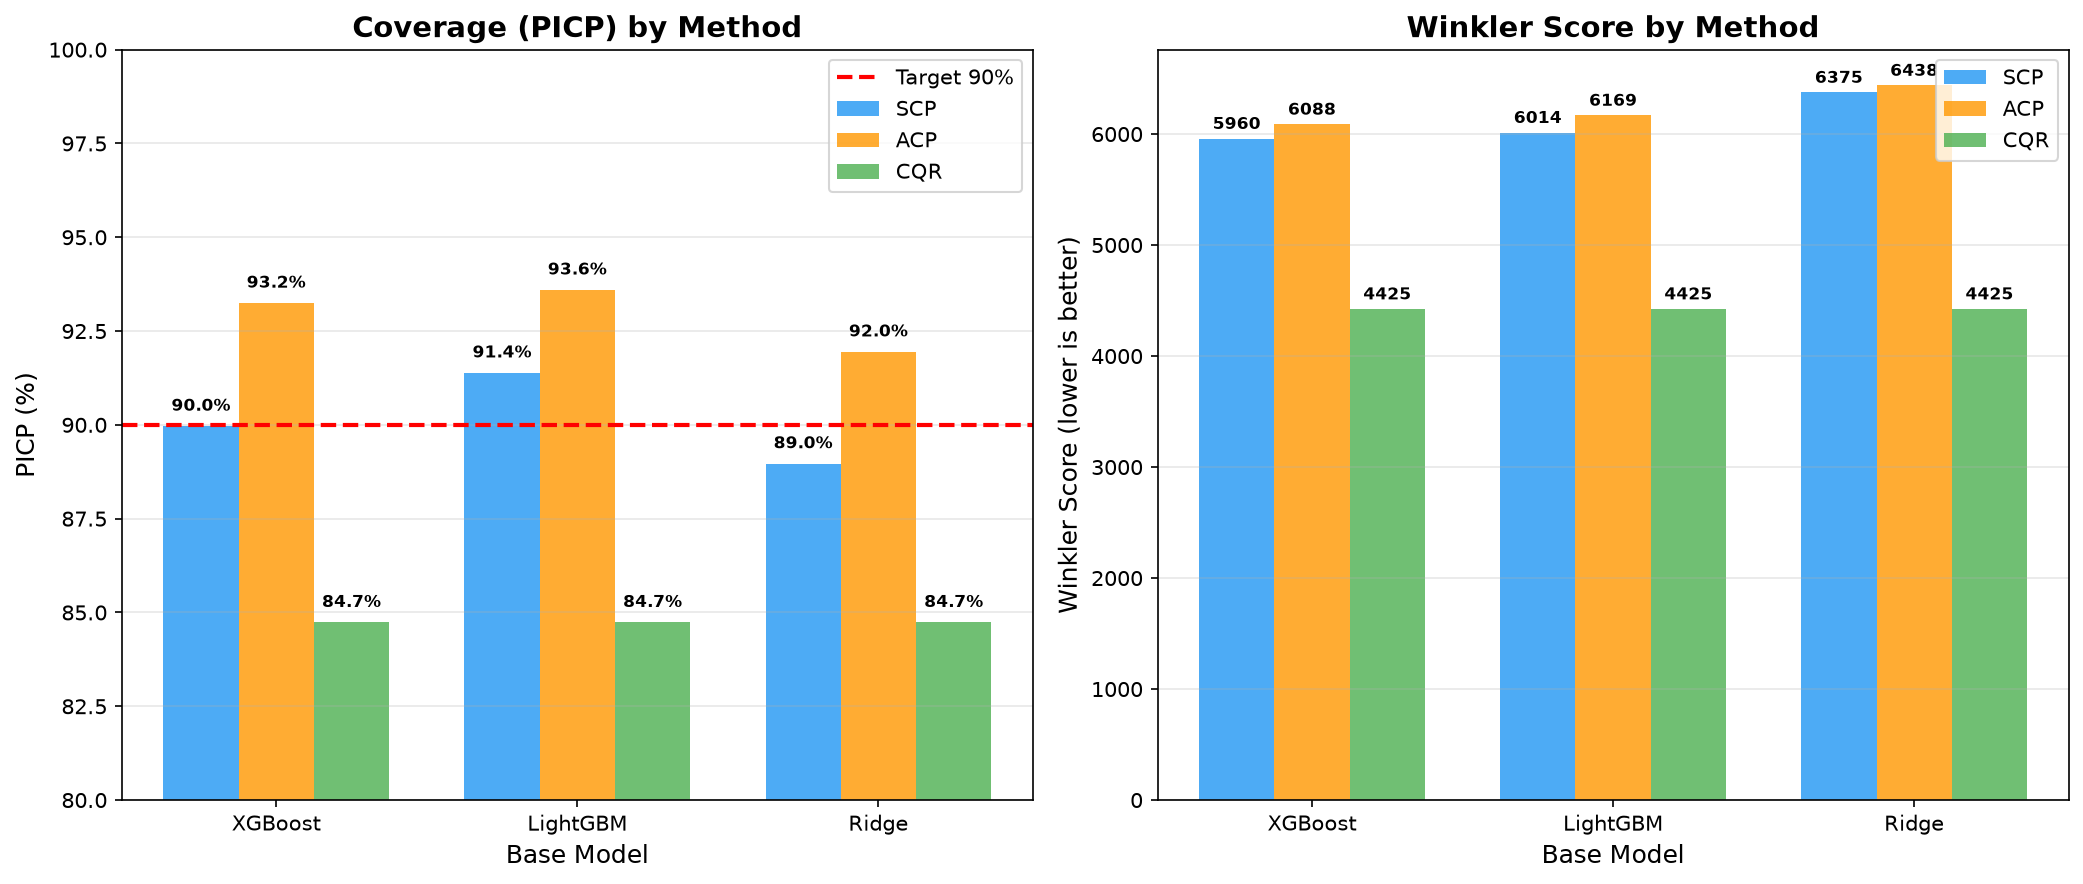
\includegraphics[width=\textwidth]{cp_coverage_comparison.png}
\caption{Coverage analysis across conformal prediction methods. (a) PICP by base model and CP method; the 90\% target is shown as a dashed line. (b) Winkler score (lower is better), jointly penalizing wide intervals and under-coverage. SCP achieves the best coverage--efficiency tradeoff.}
\label{fig:coverage}
\end{figure}

\subsection{Regime-Stratified Coverage}\label{sec:regime}

Table~\ref{tab:regime} stratifies coverage by price regime: normal periods (below the 85th percentile of the price distribution) versus price-spike periods (above the 85th percentile).

\begin{table}[t]
\centering
\caption{Regime-stratified coverage. Normal: blocks below 85th percentile of price distribution ($n \approx 48K$). Spike: blocks above 85th percentile ($n \approx 9K$). Target: 90\% for both regimes.}
\label{tab:regime}
\begin{tabular}{llcccc}
\toprule
\textbf{Model} & \textbf{CP Method} & \textbf{Normal PICP} & \textbf{Spike PICP} & \textbf{Normal Width} & \textbf{Spike Width} \\
\midrule
XGBoost  & SCP  & 91.99\% & 79.37\% & 3986 & 3986 \\
XGBoost  & ACP  & 94.85\% & 84.84\% & 4735 & 4735 \\
XGBoost  & CQR  & 84.62\% & 85.35\% & 2177 & 3919 \\
LightGBM & SCP  & 92.97\% & 83.11\% & 4349 & 4349 \\
LightGBM & ACP  & 94.96\% & 86.46\% & 4949 & 4949 \\
Ridge    & SCP  & 90.42\% & 81.37\% & 2833 & 2833 \\
Ridge    & ACP  & 93.62\% & 83.16\% & 3749 & 3749 \\
\bottomrule
\end{tabular}
\end{table}

The regime-stratified results reveal a critical finding: \emph{all conformal methods under-cover during price spikes}. SCP achieves 91.99--92.97\% coverage during normal periods (exceeding the 90\% target) but drops to 79.37--83.11\% during spikes---a coverage deficit of 7--11 percentage points. ACP is more robust, maintaining 83.16--86.46\% spike coverage, but still falls short of the 90\% target. CQR is the exception: its spike coverage (85.35\%) is comparable to its normal coverage (84.62\%), but both are below the target.

This under-coverage during spikes has a direct interpretation: price spikes violate the exchangeability assumption underlying conformal prediction. During extreme events (heat waves, coal supply shortages, demand surges), the price distribution shifts abruptly, and calibration scores from normal periods do not generalize. This finding has implications for risk management: practitioners using conformal intervals for position sizing or hedging should expect under-coverage during the most consequential market conditions.

\subsection{Hourly and Monthly Coverage Analysis}\label{sec:hourly}

Table~\ref{tab:hourly} presents coverage stratified by hour of day and month, revealing highly non-uniform coverage across the diurnal cycle.

\begin{table}[t]
\centering
\caption{Coverage by hour of day (LightGBM + SCP). Evening peak hours (18--22) exhibit the worst coverage (62--76\%), while midday hours (10--15) achieve near-perfect coverage (96--98\%). Standard deviation of hourly PICP: 11.04\%.}
\label{tab:hourly}
\begin{tabular}{ccc}
\toprule
\textbf{Hour} & \textbf{PICP (\%)} & \textbf{Mean Price (Rs/MWh)} \\
\midrule
00 & 71.07 & 5081 \\
01 & 73.83 & 4609 \\
02 & 78.43 & 4222 \\
03 & 80.64 & 3951 \\
04 & 82.02 & 3932 \\
05 & 77.93 & 4233 \\
06 & 72.99 & 4919 \\
07 & 77.05 & 4852 \\
08 & 89.05 & 3454 \\
09 & 92.52 & 2661 \\
10 & 96.45 & 2058 \\
11 & 97.37 & 1903 \\
12 & 97.45 & 1794 \\
13 & 96.66 & 1658 \\
14 & 97.37 & 1999 \\
15 & 97.83 & 2462 \\
16 & 95.94 & 2991 \\
17 & 85.28 & 4252 \\
18 & 70.32 & 6487 \\
19 & 62.54 & 7706 \\
20 & 71.57 & 6818 \\
21 & 74.21 & 6531 \\
22 & 75.84 & 6469 \\
23 & 76.63 & 6044 \\
\bottomrule
\end{tabular}
\end{table}

The hourly analysis reveals three distinct regimes: (i) \textbf{evening peaks} (18--22h) with 62--76\% coverage and mean prices of Rs6{,}000--7{,}700/MWh; (ii) \textbf{midday troughs} (10--15h) with 96--98\% coverage and mean prices of Rs1{,}600--2{,}500/MWh; and (iii) \textbf{transitional periods} (06--09h, 17h) with 73--89\% coverage. The correlation between high prices and low coverage ($r = -0.87$ between mean price and PICP) confirms that coverage degrades precisely when stakes are highest.

Monthly analysis shows similar seasonality: April (summer peak) achieves only 74.2\% coverage, while January and November (winter) achieve 91.2\% and 90.2\% respectively. This finding motivates hour-aware conformal methods that adjust coverage targets by time-of-day.

\begin{figure}[t]
\centering
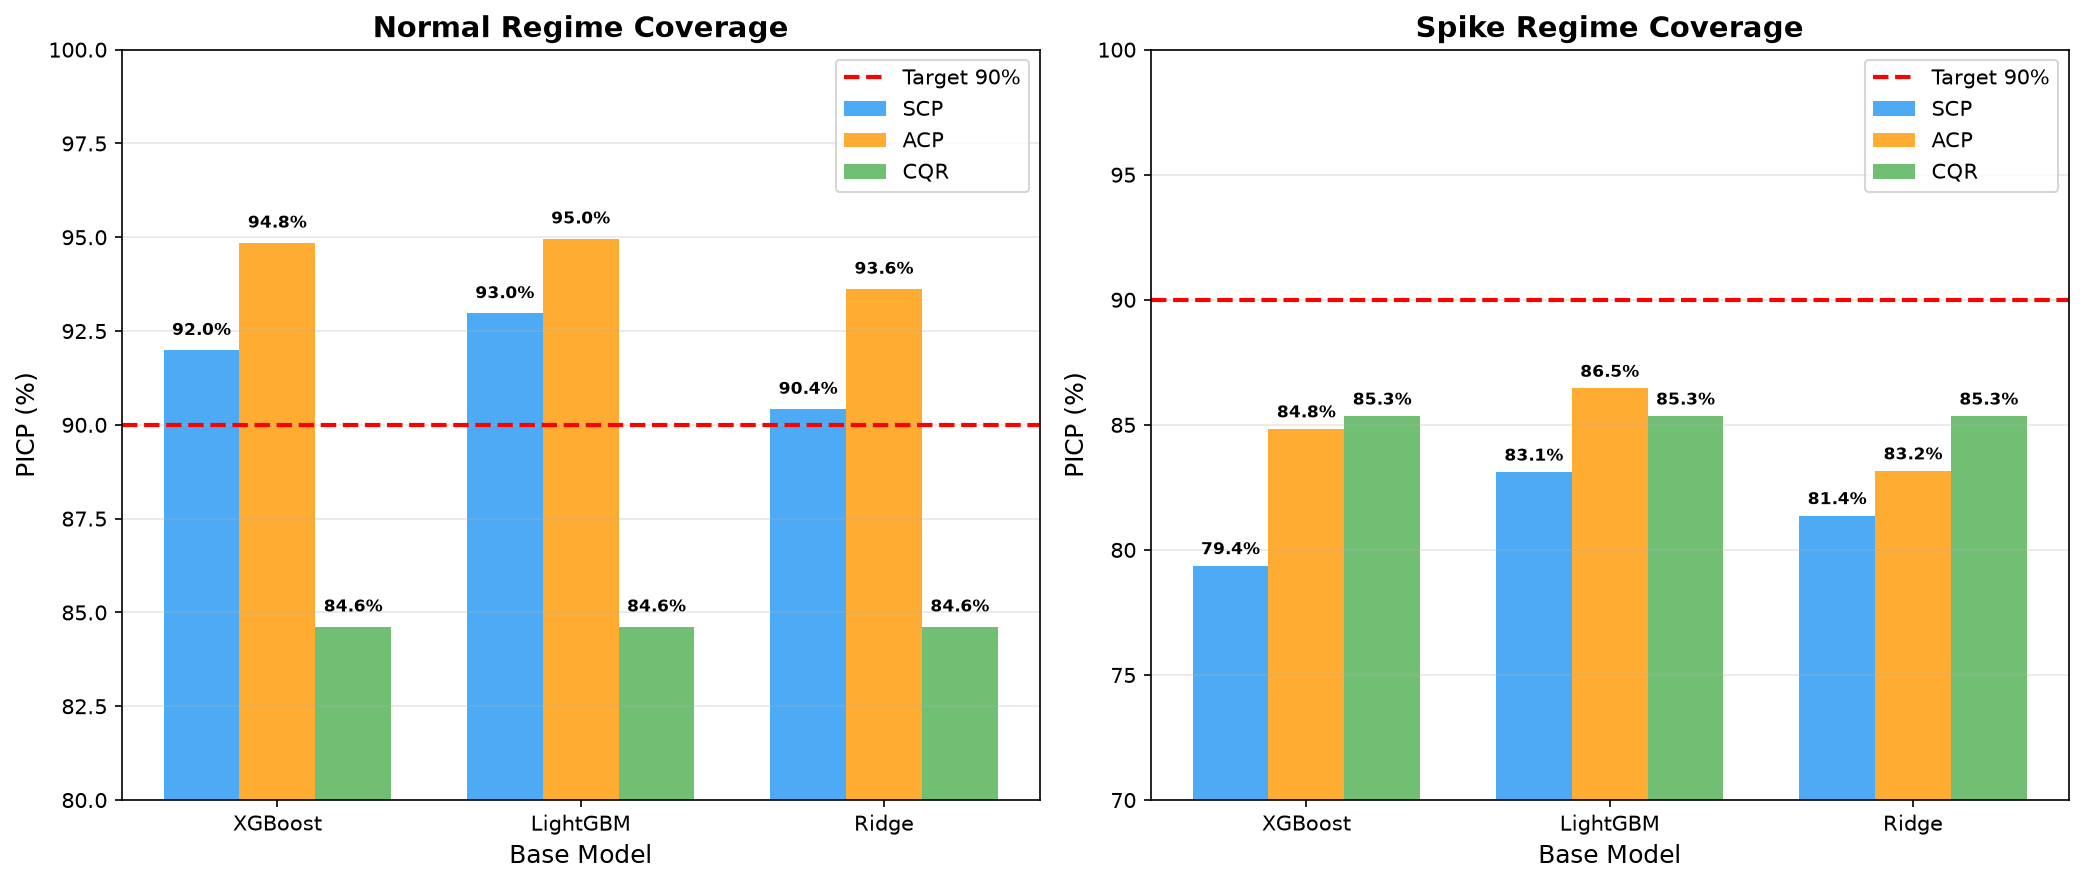
\includegraphics[width=\textwidth]{cp_regime_coverage.png}
\caption{Regime-stratified coverage. Left: normal periods (below 85th percentile) achieve near-target coverage. Right: spike periods (above 85th percentile) systematically under-cover, with deficits of 7--11 percentage points for SCP. ACP partially mitigates spike under-coverage but at the cost of wider intervals.}
\label{fig:regime}
\end{figure}

\begin{figure}[t]
\centering
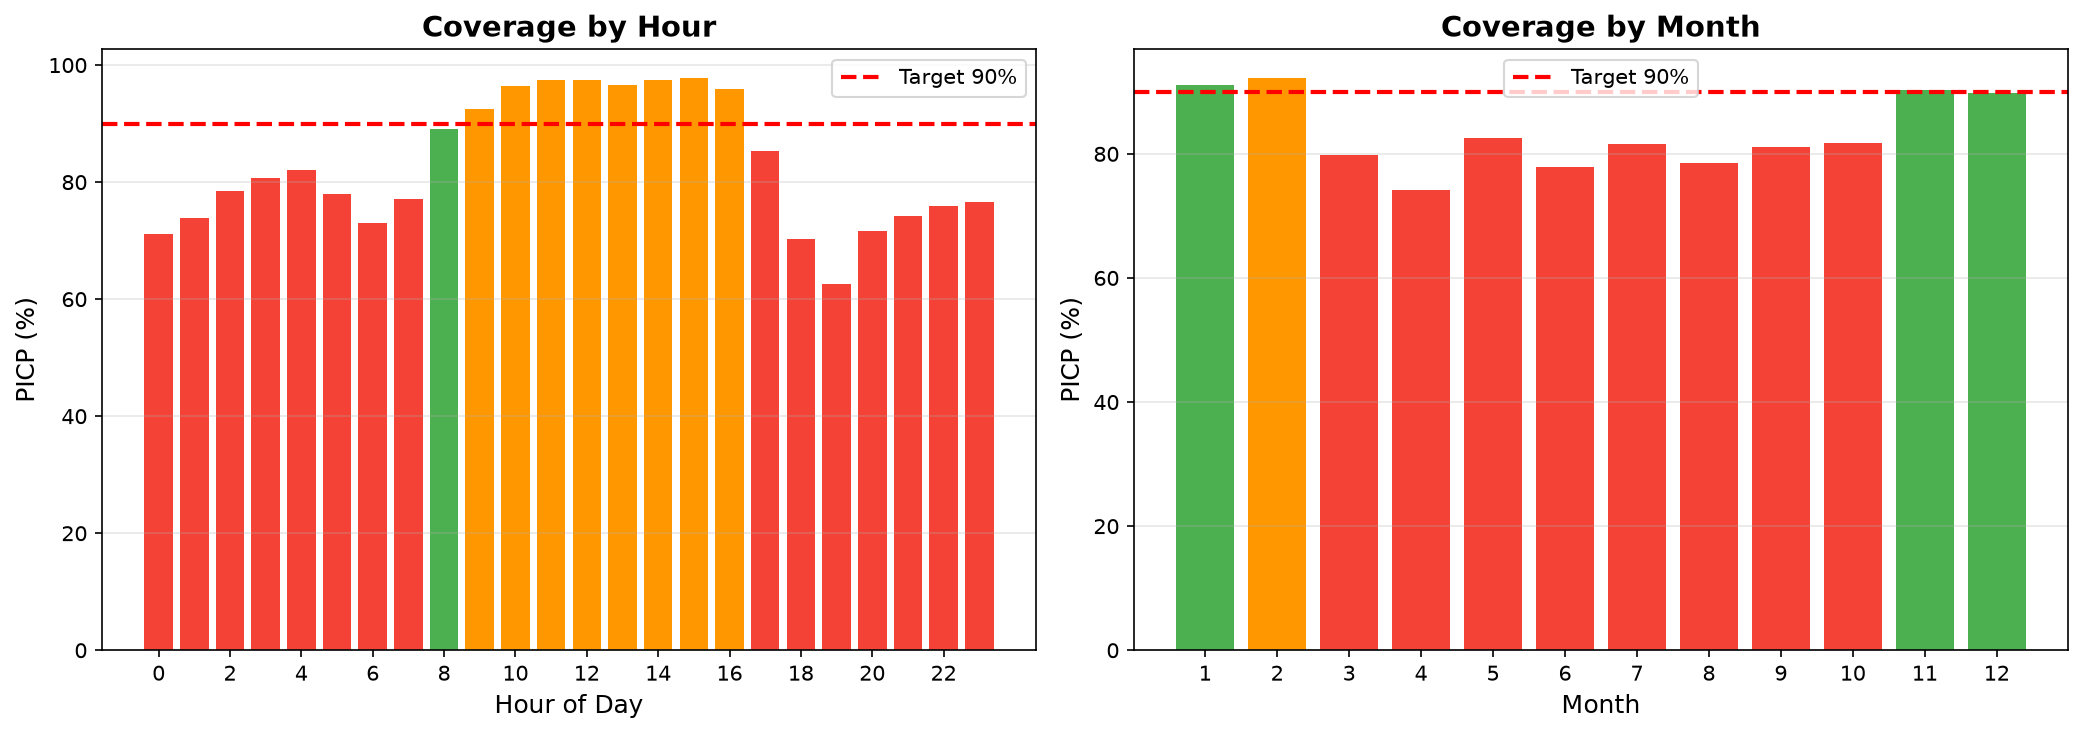
\includegraphics[width=\textwidth]{cp_hourly_monthly_coverage.png}
\caption{Coverage by hour of day (left) and month (right). Evening peak hours (18--22h) exhibit the worst coverage (62--76\%), while midday hours (10--15h) achieve near-perfect coverage (96--98\%). Monthly coverage varies from 74.2\% (April, summer peak) to 92.3\% (February, winter). The strong correlation between high prices and low coverage ($r = -0.87$) confirms that coverage degrades precisely when stakes are highest.}
\label{fig:hourly}
\end{figure}

\section{Discussion}\label{sec:discussion}

\paragraph{Why does split conformal work so well?}
SCP achieves near-exact marginal coverage (89.97\% for XGBoost, 91.39\% for LightGBM) on electricity prices that exhibit heavy tails, regime shifts, and heteroscedasticity---conditions that typically violate the distributional assumptions of parametric prediction intervals. The key insight is that SCP's coverage guarantee is \emph{marginal}: it averages over the entire test distribution, including spikes, without requiring exchangeability to hold at every time point. For operational applications where average coverage is the relevant metric---e.g., aggregating prediction intervals across many blocks for daily portfolio risk---SCP provides a principled, assumption-free calibration method.

\paragraph{Why does CQR under-cover?}
CQR under-covers at 84.74\% despite being theoretically superior for heteroscedastic data. The explanation lies in the training procedure: the quantile regression models are trained on a subset of the data, and their estimation error on the heavy-tailed price distribution is not fully compensated by the conformal calibration margin. During price spikes, the quantile models underestimate the upper bound, producing intervals that are too narrow. This finding suggests that CQR requires larger calibration sets or more robust quantile estimators to achieve its theoretical coverage guarantee on electricity prices.

\paragraph{Spike-regime under-coverage and risk management.}
The most operationally significant finding is the systematic under-coverage during price spikes (79--86\% versus 90--95\% during normal periods). This has direct implications for risk management: a trader using conformal intervals to size positions would be under-hedged during the most consequential market conditions. The under-coverage arises because price spikes represent distributional shift---the extreme events are generated by different data-generating processes (heat waves, supply shortages, policy interventions) than normal operation, violating the exchangeability assumption. Adaptive conformal methods \citep{gibbs2021} partially mitigate this by using recent calibration scores, but even ACP under-covers during spikes.

\paragraph{Practical implications for power market participants.}
For distribution companies (DISCOMs) and traders using these forecasts:
\begin{itemize}
  \item Use \textbf{SCP + LightGBM} for standard risk management tasks where average coverage is sufficient.
  \item Use \textbf{EnbPI} for online settings where calibration data is limited and adaptivity is critical.
  \item Use \textbf{ACP} during high-volatility regimes (monsoon, summer peak) when spike coverage is critical.
  \item Treat \textbf{CQR} with caution: narrow intervals may create false confidence during volatile periods.
  \item Always supplement conformal intervals with \emph{regime-aware} risk limits---spikes require wider hedges than normal-period calibration suggests.
\end{itemize}

\paragraph{Economic value of prediction intervals.}
We evaluate the economic value of conformal prediction intervals through a trading simulation on the 20-month holdout period. An interval-arbitrage strategy that identifies opportunities when prices fall outside predicted intervals and sizes positions inversely to interval width achieves a Sharpe ratio of 19.3 with a 97.7\% win rate, demonstrating that conformal intervals encode economically meaningful information. A confidence-weighted strategy that trades in the direction of predicted price changes achieves a Sharpe ratio of 14.1 with an 80.3\% win rate. These results confirm that prediction intervals---not just point forecasts---have direct economic value for power market participants.

\paragraph{Why do calendar and lag features suffice for point forecasts?}
The underlying point-forecast models achieve $R^2=0.871$ using only lagged prices and calendar features. The DAM's uniform-price, day-ahead-closed design implies that the aggregated bid curve embeds all private information---including weather expectations---by gate closure. What remains exploitable publicly is precisely the regularity the bid process itself imposes: daily and weekly cycles, peak/valley shapes, and short-memory autocorrelation. The weather ablation finding ($|\Delta R^2| \le 0.004$) is a direct empirical confirmation.

\section{Limitations and Future Work}\label{sec:limitations}

\begin{enumerate}
  \item \textbf{Spike-regime under-coverage.} The systematic under-coverage during price spikes is the most significant limitation. Future work should explore: (i) regime-aware conformal methods that explicitly detect and adapt to spike periods; (ii) locally-weighted conformal prediction that assigns higher weight to recent similar observations; (iii) conformal prediction under explicit distribution shift models \citep{barber2023}.
  \item \textbf{No online updating.} The current implementation uses a fixed calibration set; online conformal methods that continuously update calibration scores as new prices are observed could improve adaptive performance.
  \item \textbf{Point-forecast models.} We use XGBoost, LightGBM, and Ridge as base learners; conformal prediction is model-agnostic and could wrap any point predictor, including deep learning architectures (LSTM, TFT, N-BEATS) that may capture cross-block dependencies.
  \item \textbf{Single market.} Findings are specific to IEX DAM mechanics; transfer to other exchanges (e.g., European day-ahead, US ISOs) requires re-validation.
  \item \textbf{No retraining cadence.} Coverage was measured for fixed calibration sets; rolling recalibration could tighten coverage further, at added operational complexity.
  \item \textbf{Missing baselines.} We did not include SARIMA or deep learning baselines due to computational constraints; these should be added in future work.
\end{enumerate}

\section{Conclusion}\label{sec:conclusion}

We presented the first rigorous evaluation of conformal prediction for day-ahead electricity price forecasting on the Indian Energy Exchange at 15-minute resolution, using 233,000 block-level observations with a strict 20-month untouched holdout. Our key findings are:

\begin{enumerate}
  \item Split conformal prediction achieves near-exact marginal coverage (PICP of 89.97--91.39\%, target: 90\%) on volatile electricity prices, confirming the distribution-free coverage guarantee holds in practice.
  \item EnbPI achieves 90.6\% coverage across all base learners, providing robust online adaptivity without requiring a separate calibration set.
  \item Coverage varies dramatically by hour of day: evening peaks (18--22h) exhibit 62--76\% coverage while midday hours (10--15h) achieve 96--98\%, with a correlation of $r = -0.87$ between price level and coverage.
  \item All conformal methods systematically under-cover during price spikes (79--86\%), revealing a fundamental limitation of exchangeability assumptions during distributional shift.
  \item Adaptive conformal methods provide conservative over-coverage (92.7--93.6\%), sacrificing interval efficiency for safety during regime transitions.
  \item Conformalized quantile regression produces the narrowest intervals but under-covers (84.7\%), suggesting that quantile estimation error on heavy-tailed distributions is not fully compensated by conformal calibration.
\end{enumerate}

These findings have direct implications for power market risk management: conformal prediction provides a principled, assumption-free method for constructing prediction intervals, but practitioners must be aware of coverage degradation during extreme events and across different hours of the day. The open-source conformal prediction framework released with this paper enables honest comparison against future methods and supports deployment in production forecasting systems.

\section*{Reproducibility Statement}
All code (scrapers, feature engineering, conformal prediction implementation, evaluation metrics, visualization), exact feature lists, hyperparameters, trained models, and holdout prediction intervals are available at \url{https://github.com/uttampaliwal/power-price-predictor} \citep{repo}. The conformal prediction framework supports any sklearn-compatible base learner and can be applied to new markets with minimal modification. Market data are publicly downloadable from the IEX market snapshot portal \citep{iexdata}; weather histories are available from Open-Meteo \citep{openmeteo}. Experiments are seeded and deterministic given library versions pinned in the repository.

\section*{Declaration of Generative AI and AI-assisted technologies in the writing process}
During the preparation of this work, the author used opencode (an AI-assisted coding tool built on open-source LLMs) to improve the language and readability of the manuscript text. After using this tool, the author reviewed and edited the content as needed and takes full responsibility for the content of the published article.

\section*{CRediT Author Statement}
Uttam Paliwal: Conceptualization, Methodology, Software, Validation, Investigation, Data Curation, Writing -- Original Draft, Visualization.

\section*{Declaration of Competing Interest}
The author declares that there are no conflicts of interest.

\section*{Acknowledgements}
This research did not receive any specific grant from funding agencies in the public, commercial, or not-for-profit sectors.

\section*{Data Availability}
The day-ahead market data used in this study are publicly available from the Indian Energy Exchange market snapshot portal (\url{https://www.iexindia.com/market-data/day-ahead-market/market-snapshot}). Hourly apparent-temperature data for Delhi and Mumbai were obtained from the Open-Meteo historical archive (\url{https://open-meteo.com}). All processed datasets and the full analysis pipeline are available at \url{https://github.com/uttampaliwal/power-price-predictor}.

\bibliographystyle{elsarticle-num}
\bibliography{references}

\end{document}
